\documentclass[conference]{IEEEtran}
\usepackage{caption}
\IEEEoverridecommandlockouts
% The preceding line is only needed to identify funding in the first footnote. If that is unneeded, please comment it out.
\usepackage{cite}
\usepackage{amsmath,amssymb,amsfonts}
\usepackage{algorithmic}
\usepackage{graphicx}
\usepackage{stfloats} % For better control of float placement

% for multiple image adding
\usepackage{caption}
\usepackage{graphicx}
\usepackage{subcaption}



\hyphenation{op-tical net-works semi-conduc-tor}



\begin{document}

% \title{Toward a Multi-Agent Approach for Dynamic Traffic Control and Optimization}

\title{Toward a Multi Agent Approach for LLM-Based Dynamic Vehicle Control and Communication in Accidental Condition}

% author names and affiliations
% use a multiple column layout for up to three different
% affiliations
\author{\IEEEauthorblockN{Rafi Md Ashifujjman}
\IEEEauthorblockA{\textit{Graduate School of}\\
\textit{Integrated Science and Technology}\\
\textit{Shizuoka University}\\Hamamatsu, Japan\\ rafi.md.ashifujjman.23@shizuoka.ac.jp}
\and

\IEEEauthorblockN{Naoki Fukuta}
\IEEEauthorblockA{\textit{College of Informatics, Academic Institute}\\
\textit{Shizuoka University}
\\Hamamatsu, Japan\\fukuta@inf.shizuoka.ac.jp}}

\maketitle
%done with tittle means name , author , etc.

% in the abstract
\begin{abstract}
% In autonomous vehicles (AVs), making the right decision in unknown traffic situations remains a challenge. Traditional AVs rely on pre-trained models, which often struggle in such cases where human-like reasoning is required. In this research, we examine how Large Language Models (LLMs) act as a decision agent responding to scenario-specific text prompts derived from real-world traffic situations. In addition, we propose a `Communication Agent' that enables vehicle-to-vehicle (V2V) information sharing, such as speed, obstacles, and future intentions, in a structured format to provide contextual support for the decision agent.This paper proposes a preliminary approach to assess whether LLMs within a multi-agent framework, when provided with structured prompts and contextual data (unknown traffic situation), can support consistent and human-like decision making.

In autonomous vehicles (AVs), making the right decision in unknown traffic situations remains a challenge. Traditional AVs rely on pre-trained models, which often struggle in such cases where human-like reasoning is required. In this research, we examine how Large Language Models (LLMs) act as a decision agent responding to scenario-specific text prompts derived from real-world traffic situations. In addition, we propose a `Communication Agent' that enables vehicle-to-vehicle (V2V) information sharing, such as speed, obstacles, and future intentions, in a structured format to provide contextual support for the decision agent.This paper proposes a preliminary approach to assess whether LLMs within a multi-agent framework, when provided with structured prompts and contextual data, can support consistent and human-like decision making.
\end{abstract}

\begin{IEEEkeywords}
autonomous vehicles, large language models (LLMs), multi-agent, vehicle-to-vehicle (V2V) communication, decision making agent, communication agent.

\end{IEEEkeywords}

\IEEEpeerreviewmaketitle



\section{Introduction}

This paper explores the potential of integrating Large Language Models (LLMs)\cite{chang2024survey} into a multi-agent framework\cite{10707898} to improve decision making in autonomous vehicles (AVs), particularly in unknown and unsafe traffic situations.
Our main concern would be to explore the use of LLMs for autonomous driving systems (ADS) as the main decision-making agent within a multi-agent framework to evaluate its reasoning ability\cite{10707968} to handle uncertain traffic situations. Our goal is to contribute to the development of safer and more reliable Level 5\cite{cho2020more} autonomous vehicles. We aim to contribute for level 5 (complete automation \cite{raza2018autonomous}). There are numerous instances in which traditional autonomous vehicles are capable of making effective decisions in familiar scenarios using pre-trained models.  However, they may have trouble facing new or unusual situations where their programmed knowledge is not directly covered in such situations. Human drivers can use common sense and past experiences to handle unexpected events, such as knowing that traffic cones on a moving truck are not dangerous. However, current AV systems, even those that use rule-based approaches or reinforcement learning (RL\cite{kaelbling1996reinforcement}), will struggle in these scenarios. This limitation is especially evident in what we call unknown-unsafe domain situations where the correct action is not immediately clear \cite{fu2024drive}.
During this investigation with various LLMs, we proceed our investigation under two assumptions: 1) certain AIs can transform real-world situations into text-based explanations, which are subsequently used as input for the LLMs, and 2) the outputs generated by the LLMs can be translated into actual decisions made by the AV’s decision agent by interpreting the responses from the LLMs. We are investigating the effectiveness of various LLMs for use as decision-making agents in autonomous driving systems. Our initial objective is to answer the research question (Research Question 1): Can an agent make decisions with the help of an LLM without undergoing a specific learning process for each new situation?
In our research, we will assume that vehicle-to-vehicle (V2V) communication has been achieved through a standardized networking protocol, such as LAN-based direct communication or a low-latency wireless system. Under this assumption, each vehicle can communicate with other vehicles within a defined radius (e.g., 10 meters). When a vehicle enters the information sharing radius of another vehicle, it can exchange data regarding their current status, such as obstacle detection, traffic conditions, direction, and future intended actions.
To evaluate the impact of V2V communication on autonomous decision-making, we will investigate how LLMs process and utilize this information. Specifically, we will examine whether the incorporation of V2V exchanged data improves decision accuracy and enables AVs to make more precise and context-aware decisions.
However, V2V communication introduces a critical question, (Research Question 2): Is a single centralized decision-making agent sufficient to process all incoming V2V data and make autonomous driving decisions, or is a multi-agent system required for improved efficiency and scalability? In this paper, we investigate the answers to these two research questions. 


\begin{figure}[!h]
    \centering
    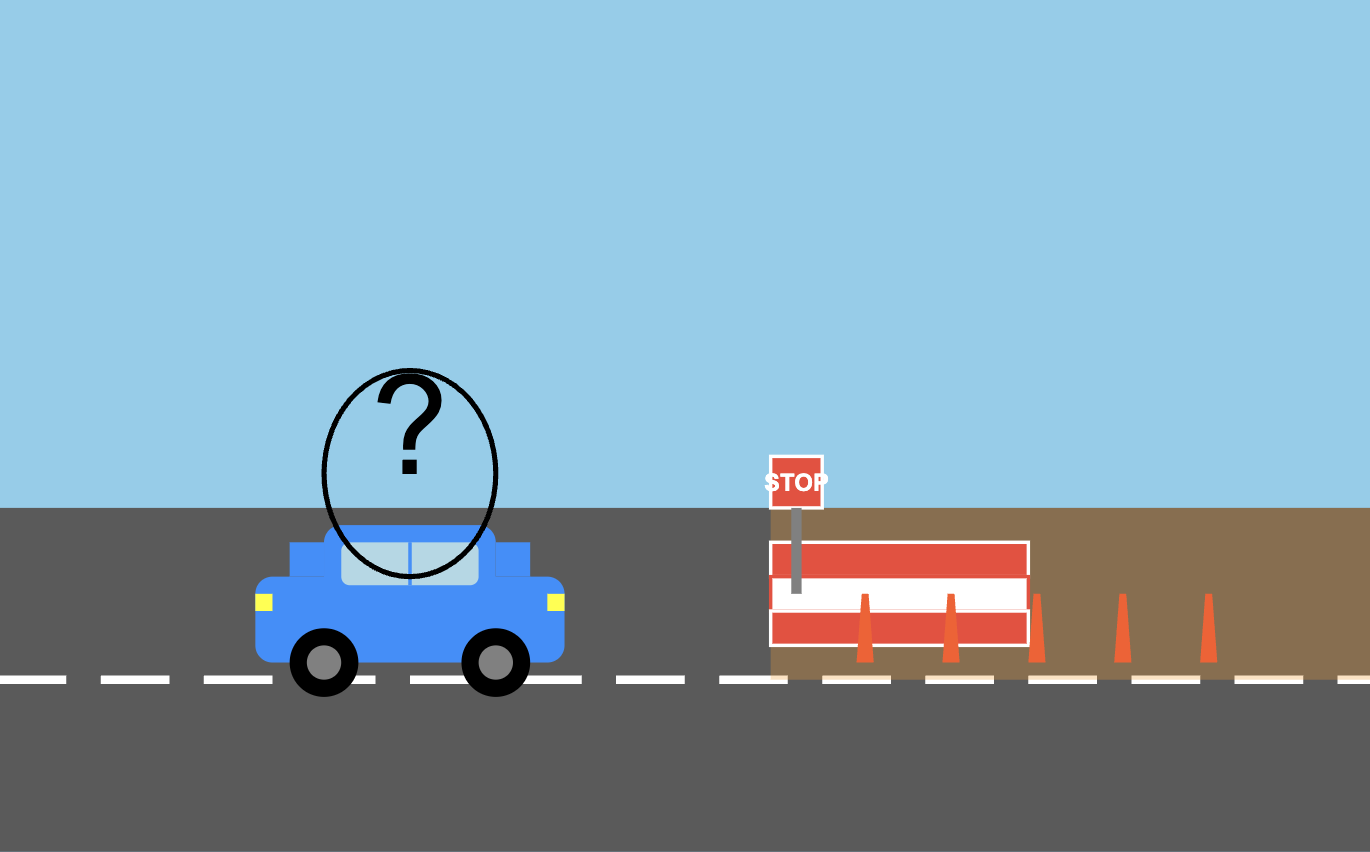
\includegraphics[width= \linewidth]{s2.png}
    \caption{What current AV might do in this situation?}
    \label{fig:enter-label-unique}
\end{figure}
\section{Motivation and Background}

Imagine a traffic situation, where a road is partially blocked due to construction, with traffic cones and a `STOP' sign indicating a partial road block. A typical autonomous vehicle (AV) might see the `STOP' sign and interpret it as a complete road closure, coming to a complete stop because that is what its pre-programmed data tell it to do. However, a human driver in the same situation might use common sense, realize that the road is only partially closed, and safely continue through the open section.

\begin{figure}[ht]
    \centering
    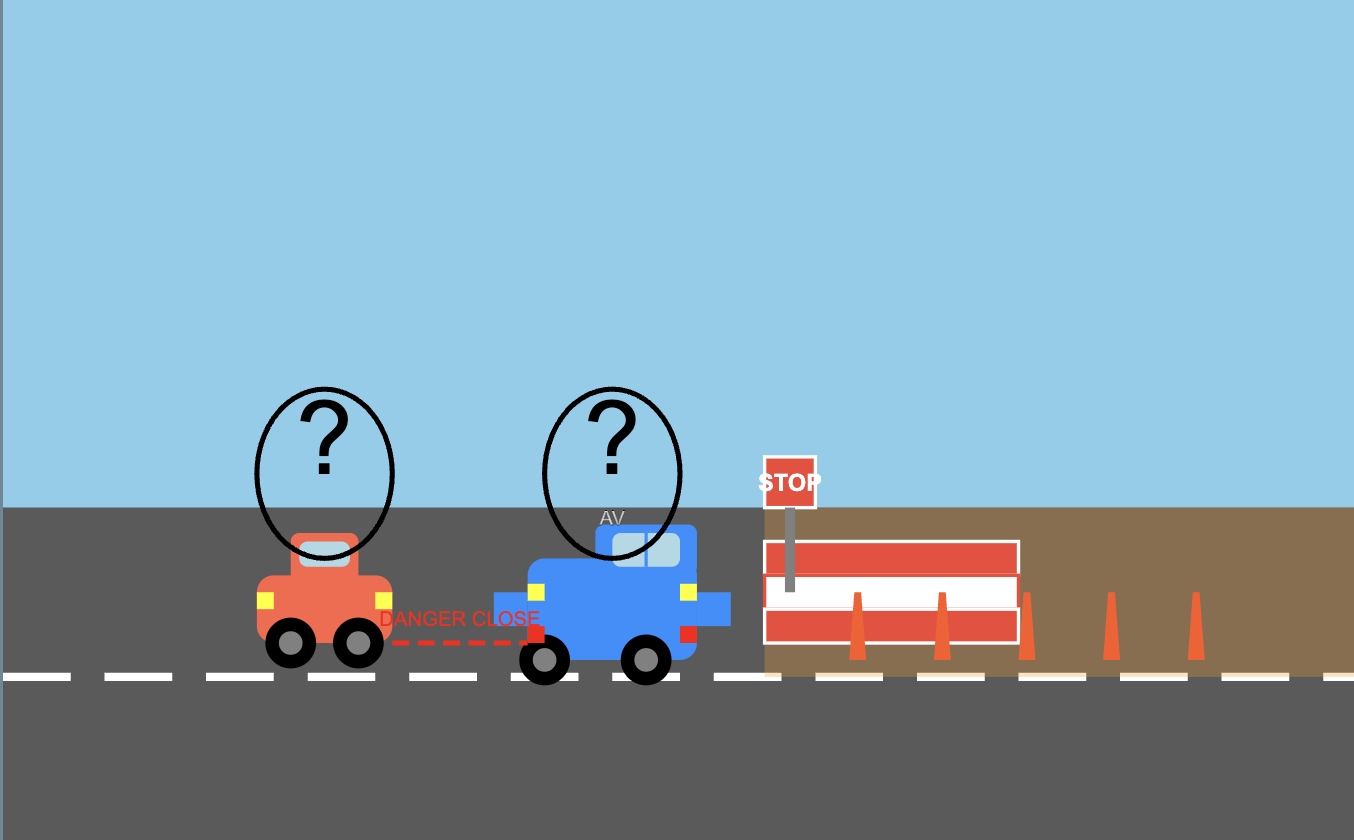
\includegraphics[width= \linewidth]{s1.png}
    \caption{Lack of communication between vehicles may lead to a potential accident.}
    \label{fig:enter-label-unique-2}
\end{figure}

Now imagine a more complicated situation where an autonomous truck comes to a sudden stop when it sees the `STOP' sign. There is another car, driven by a human or another AV, right behind it. This sudden stop could easily cause a crash. 
Now imagine a human driver encountering a partially blocked road. To navigate safely, the driver shifts into the adjacent open lane, relying on instinct, experience, and situational awareness. Anticipating the possibility of an oncoming vehicle from the opposite direction or from behind, the driver would proactively slow down, assessing the risk, and would take the necessary precautions to avoid a collision. In contrast, a traditional AV, which lacks human-like reasoning and predictive thinking, may not recognize the potential danger. Without contextual understanding, it can continue at its normal speed, assuming the lane is clear, increasing the risk of a head-on collision.

However, if the AV had better reasoning abilities, it might recognize that the road is only partially closed and proceed safely through the open part. And if the AV could communicate with the vehicle behind it, it could alert the other driver about its intended actions, particularly if the lane were to close suddenly, helping to prevent a potential accident.
A fundamental challenge in traditional autonomous vehicles (AVs) is to prepare for all truly unknown situations\cite{singh2024systematic}. Any scenario we create is technically `known' to us, even if it feels unfamiliar to the AVs, making it difficult to test how AVs handle truly unknown-unsafe situations. In addition, it is difficult to recreate complex real-world scenarios in simulation environments. For example, it is difficult to accurately simulate unpredictable human actions or complicated environmental conditions. In real life, there could be countless unexpected situations that are nearly impossible to include in training data sets for traditional autonomous driving systems (ADS) to avoid accidents. Human drivers use common sense to deal with these situations, so through this research we will explore whether LLMs can also show human-like reasoning to handle them effectively or not. 

To address these challenges, we propose a possible approach on integrating LLMs into a multi-agent framework for autonomous driving control system. LLMs have the potential to provide common sense or reasoning ability that traditional systems lack, helping AVs better understand the context of complex real-world scenarios. Incorporating Vehicle-to-Vehicle communication using multi-agent, which will allow vehicles to exchange information with other vehicles. This capability is also essential for creating realistic and complex driving scenarios.

\section{Preliminary}
% Reasoning is a fundamental aspect of human intelligence, essential for problem solving, decision-making, and critical thinking. In recent years, Large Language Models (LLMs) have demonstrated emergent abilities\cite{wei2022emergent}, such as in-context learning\cite{dong2022survey}, role play\cite{shanahan2023role} and analogical reasoning\cite{wei2022chain}. These abilities allow LLMs to go beyond natural language processing problems to facilitate a wider range of tasks, such as code generation\cite{gehring2024rlef}, robotic control\cite{ahn2022can}, and autonomous agents\cite{deng2023mind2web}. Among these abilities, human-like reasoning has garnered significant attention from both academia and industry, since it demonstrates great potential for LLMs to generalize to complex real-world problems through abstract and logical reasoning. A notable breakthrough in this area is the 'chain of thought' prompting technique\cite{wei2022chain}, which can elicit step-by-step human-like reasoning processes at test time without any additional training. 
\begin{figure}[h]
    \centering
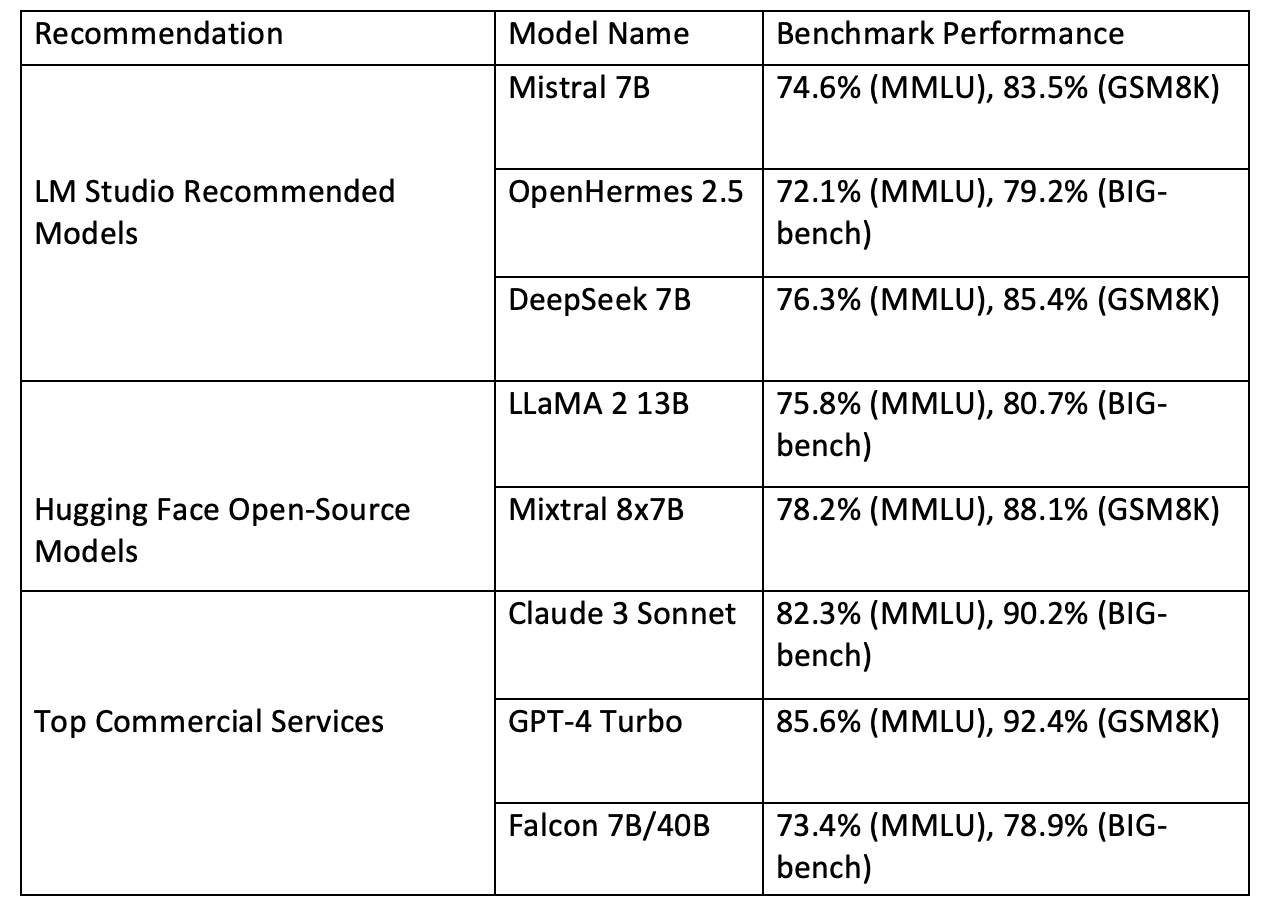
\includegraphics[width=\linewidth]{Fig/Selected_LLM.png}
    \caption{Selected Models for the Experimentation}
    \label{fig:enter-label}
\end{figure}

% \clearpage % This helps force the figure to the bottom
\begin{figure*}[h] % You already had the [b] which is correct
    \centering
    % First Row
    \begin{subfigure}[b]{0.3\textwidth}
        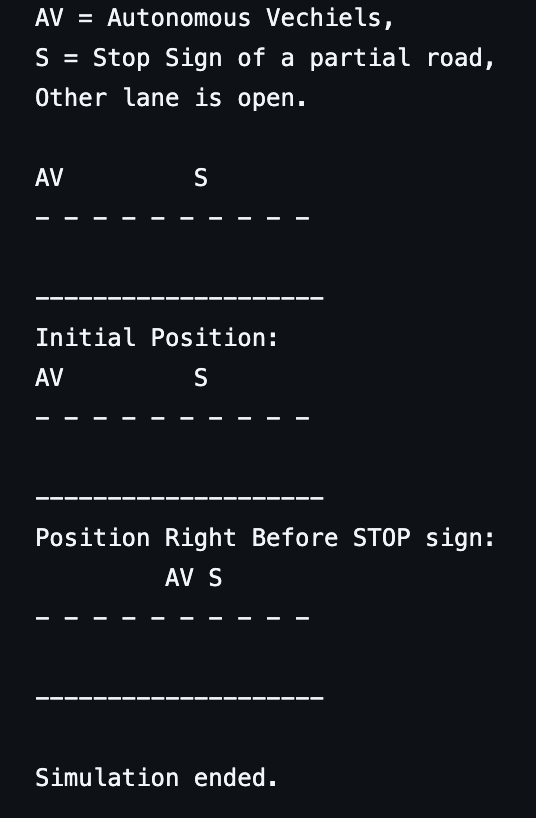
\includegraphics[width=\linewidth]{Fig/PL_Stop_S1.png}
        \caption{Stop sign on Partial road}
    \end{subfigure}
    \hfill
    \begin{subfigure}[b]{0.3\textwidth}
        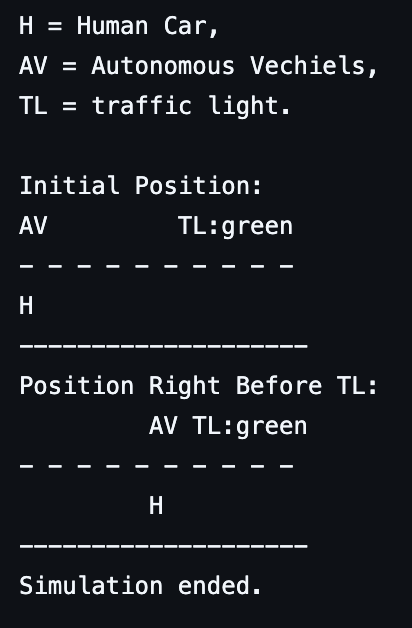
\includegraphics[width=\linewidth]{Fig/Commonsense_S2.png}
        \caption{Traffic Light}
    \end{subfigure}
    \hfill
    \begin{subfigure}[b]{0.3\textwidth}
        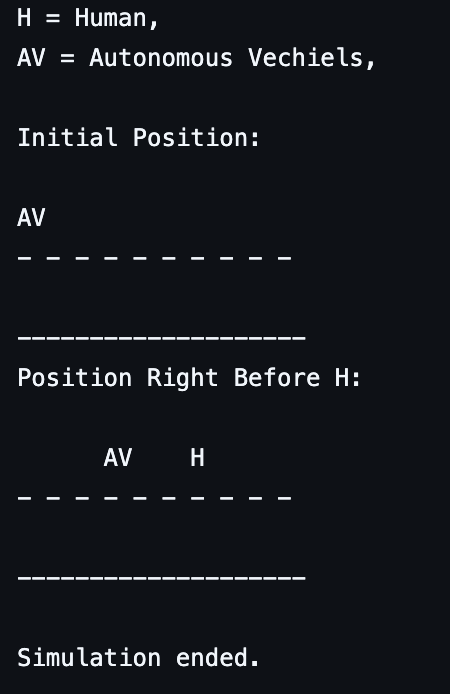
\includegraphics[width=\linewidth]{Fig/Human_reasoning_S3.png}
        \caption{Human suddenly crossing road}
    \end{subfigure}
    \caption{Illustration of real life traffic scenarios}
    \label{fig:llm_outputs}
\end{figure*}


% \textbf { Can LLMs effectively enhance decision making for AVs in Unknown-Unsafe domains within a multi-agent framework compared to current mechanisms?}
Hugging Face\footnote{https://huggingface.co/} is a platform where various open LLM models are available. LM Studio\footnote{https://lmstudio.ai/} is a platform to test and integrate LLM available on Hugging Face into a locally available system on ordinary computing devices, even without powerful GPUs. Now, the question is what factors were considered in the selection of LLMs for this study? One key factor in our model selection was quantization, which optimizes model performance while reducing computational requirements. This research \cite{xiao2023smoothquant} indicates that 8-bit quantization enables the majority of LLMs to maintain a performance level comparable to their nonquantized equivalents, regardless of model size (e.g. 7B to 70B parameters). Moreover, LLMs that are quantized to 4 bits can also up hold similar performance to their non-quantized versions across most benchmarks. This approach achieves memory reduction of 50 to 75\% while preserving precision in complex tasks such as reasoning, decision making, and domain-specific applications. 
The models chosen for this investigation were selected using a structured approach based on three key factors: popularity and performance in text-to-text generation, LM Studio recommendations for optimized accuracy, and comparative evaluations of the top commercial services. Specifically, 1) Some models were chosen based on the highest number of downloads from Hugging Face, ensuring widespread adoption and benchmark effectiveness. 2) Models suggested by LM Studio were included due to their strong performance and compatibility with local inference environments. 3) The best commercial services were selected based on their comparative performance with open-source counterparts, prioritizing accuracy, interpret ability, and real-time inference. The selected models are shown in Fig. 3. However, not all Hugging Face models are fully compatible with the LM Studio runtime. As a result, some models were tested directly on the Hugging Face interface to avoid compatibility issues. Furthermore, while models such as OpenAI’s o1, DeepSeek R1, and Llama 3.1 405B have demonstrated strong benchmark performance, they were not included in this study due to limited quantization support, lack of local deployment feasibility, and restricted open-source availability.

% ( comment: In reality, there could be countless unexpected situations in traffic scenarios that are nearly impossible to include in training data sets for traditional autonomous driving systems. Through this research we will explore whether LLMs can show human-like reasoning to avoid any accident. We have make a simulation using python to create these text base scenarios and create 7 scenarios for now. some of them are very basic like AV is hitting obstacle. how many situation i have to make or can i only mention about 4 scenarios that covers both, Complex situations and Common Knowledge Scenarios) 


To test these selected models, we have prepared a set of simple text-based simulation scenarios using Python, as illustrated in Fig. 4. These scenarios are designed to cover situations that require logical reasoning or the application of common rules knowledge, such as recognizing a red traffic light and stopping accordingly. These scenarios will be used as input for various LLMs to assess how effectively they handle both types of challenges. The experiments will be conducted using the LLM selected in Fig.3. 


% we seled a straightforward scenario featuring an autonomous vehicle (AV) approaching a green traffic light, as illustrated in Figure 4(a). The scenario was presented to selected LLMs using the prompt: "What the AV car on the above would do? Please just answer  STOP or FORWARD." We systematically ran these scenarios across different models including Claude 3.7 Sonnet, GPT-4-turbo, and open-source models such as  OpenHermes-2.5-Mistral-7B and google/flan-t5-large, as shown in Fig.6.
% The responses from the models provided by Hugging Face, LM Studio suggestions, and commercial services are shown in Figure 6. The purpose was to assess whether the models could accurately recommend actions based on the complexity and ambiguity of each scenario.





% The chosen models are shown in Fig. 4. One thing to note is that not all the models available on Hugging Face are compatible with the LM Studio runtime. Therefore, we ran some of the chosen models from Hugging Face on the Hugging Face interface itself due to compatibility issues.The models used for this investigation are selected in three ways: 1. Some text-to-text generation models have been chosen based on the highest number of downloads from Hugging Face, 2. The models suggested by LM Studio are considered as they offer best performance and accuracy, 3. The top commercial services that are openly available are taken into account on the basis of the performance evaluation with other commercial services. The chosen models are shown in Fig. 4. One thing to note is that not all the models available on Hugging Face are compatible with the LM Studio runtime. Therefore, we ran some of the chosen models from Hugging Face on the Hugging Face interface itself due to compatibility issues.


% For each scenario, we asked the same question to each language model at least 20 times. The purpose was to check whether the model could give the same answer every time or if its decision would change. This helps us understand how consistent and reliable the models are when used in critical tasks like deciding whether an autonomous vehicle should "STOP" or "FORWARD" in difficult situations.


% In our research, we will create specific scenarios and use them as inputs for LLM to see if they can demonstrate human-like reasoning in unknown unsafe situations. By examining how well LLMs can handle these scenarios, our objective is to determine whether they can improve the current struggles faced by AVs.
% We will run this test on various cloud base and local base LLM.

% To address this, we will design various custom scenarios requiring logical reasoning or common knowledge (e.g., stopping at a red light) and use them as inputs to different LLMs. By evaluating how well these models navigate such situations, we aim to assess their potential to overcome the challenges faced by current AV systems. These experiments will be conducted using cloud-based and locally deployed LLMs.


% Now lets introduce the output from different LLM and disscuss about the input and also i gonna disscuss about the assumption.

% \begin{figure}[h]
%     \centering
%     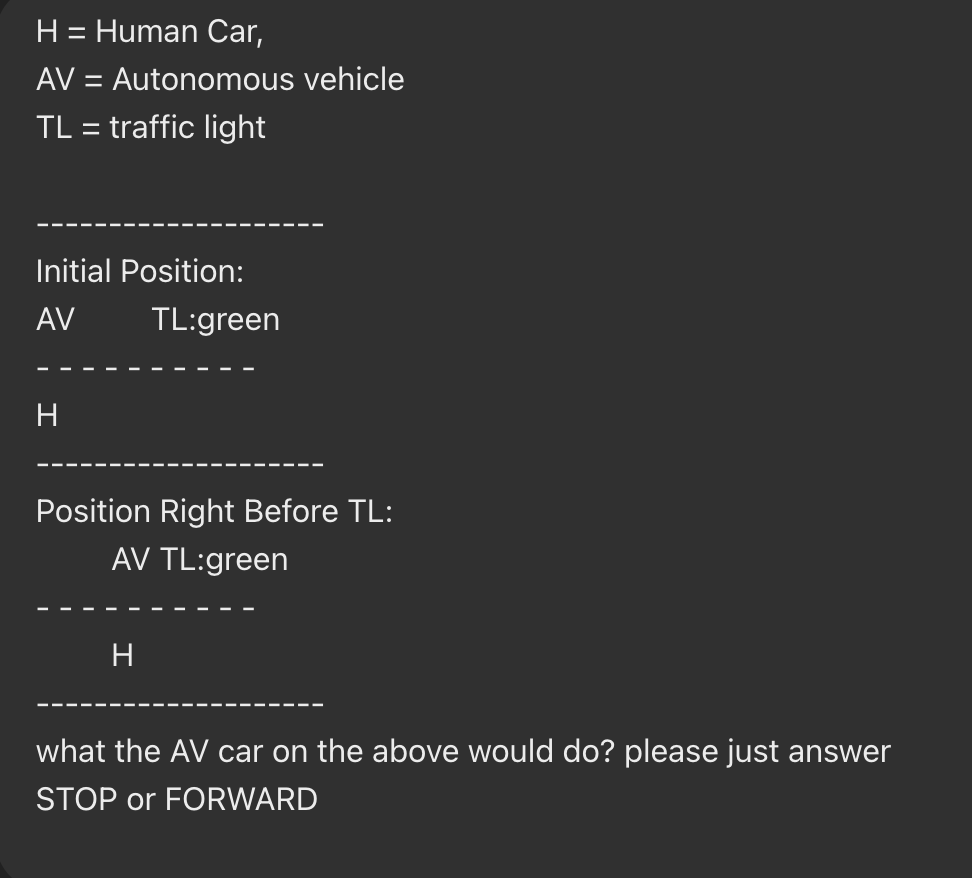
\includegraphics[width= \linewidth]{Scenario.png}
%     \caption{Text-base scenario}
%     \label{fig:enter-label}
% \end{figure}



% Several scenarios representing both "known-safe" and "unknown-unsafe" situations, where decision-making may be straightforward or ambiguous for autonomous vehicles, were presented to various language models. These scenarios were converted into text-based natural language prompts to simulate real-world decision-making challenges. For consistency, we added the instruction: "What should the AV do in the above situation? Please, just answer with 'STOP' or 'FORWARD'." 

% For each test scenario, we have queried each model at least 20 times to assess consistency and determine whether the model could reliably produce the same result in multiple runs.We presented a text-based scenario showing the autonomous vehicle (AV) and human-driven car (H) approaching a green traffic light similar to the one in Fig. 4, to the language models. We used the following prompt: What would the AV do in this situation? Please, just answer STOP or FORWARD. We ran this same prompt at least 20 times in OpenHermes-2.5-Mistral-7B and analyzed the results.

 % \begin{figure}[h]
 %     \centering
 %     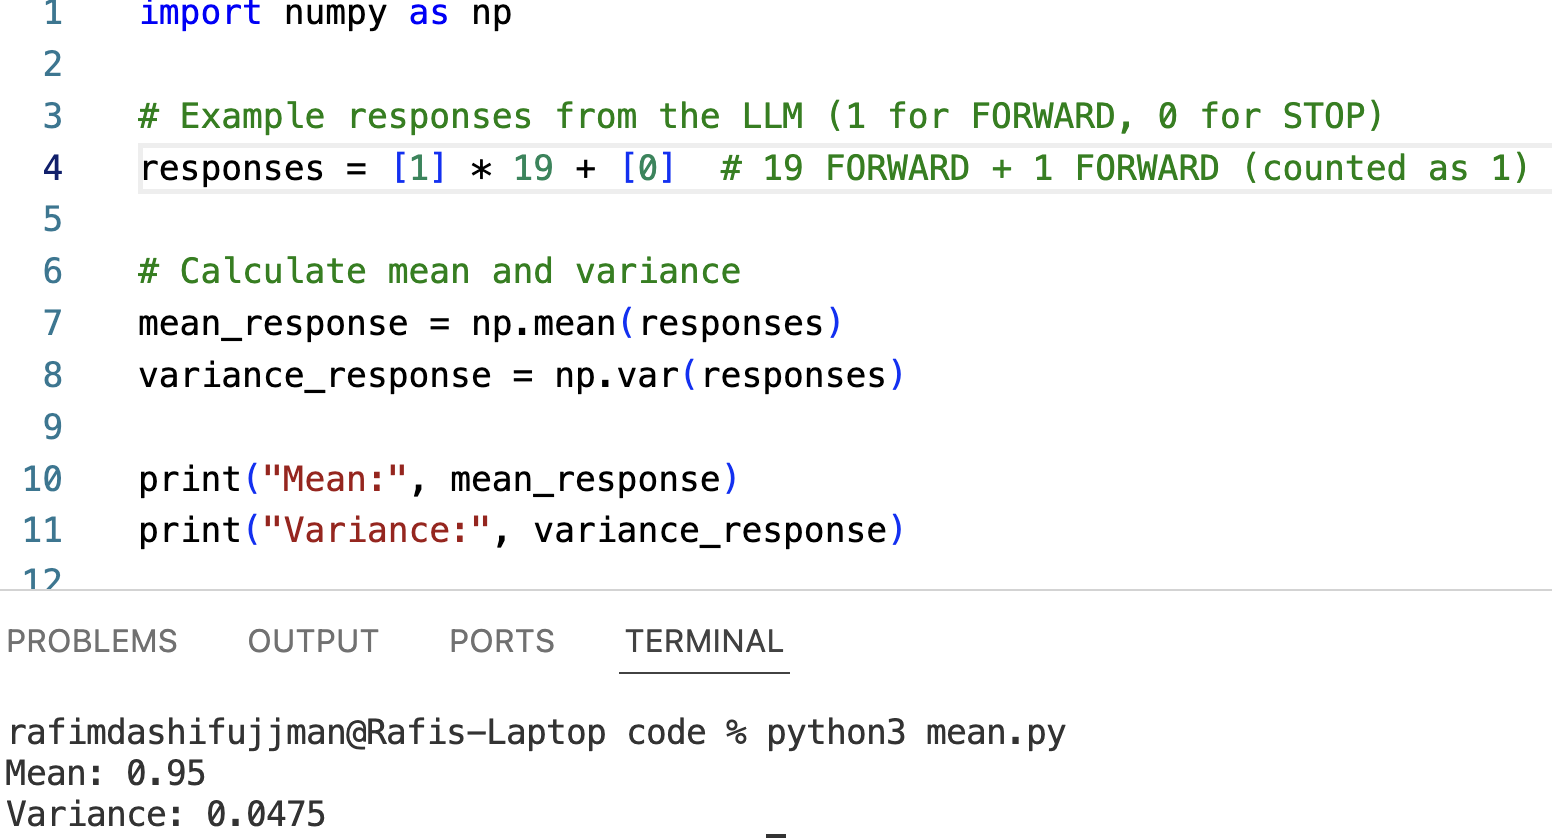
\includegraphics[width=\linewidth]{Fig/mean.png}
 %     \caption{LLM Model Response Analysis}
 %     \label{fig:enter-label}
 % \end{figure}
 

 


\section{Our Approach}
The main phase of this research focuses on using the shared data of the communication agent within our proposed multi-agent framework. The `Communication Agent' ensures that vehicles share critical information, including obstacle detection, traffic conditions, speed, and intended actions, in a standardized format within a defined radius, the expected format is demonstrated in Fig. 5. This structured data exchange is expected to significantly improve the accuracy of `Decision Agent' by providing a more comprehensive contextual understanding of the driving environment.
 \begin{figure}[!ht]
     \centering
     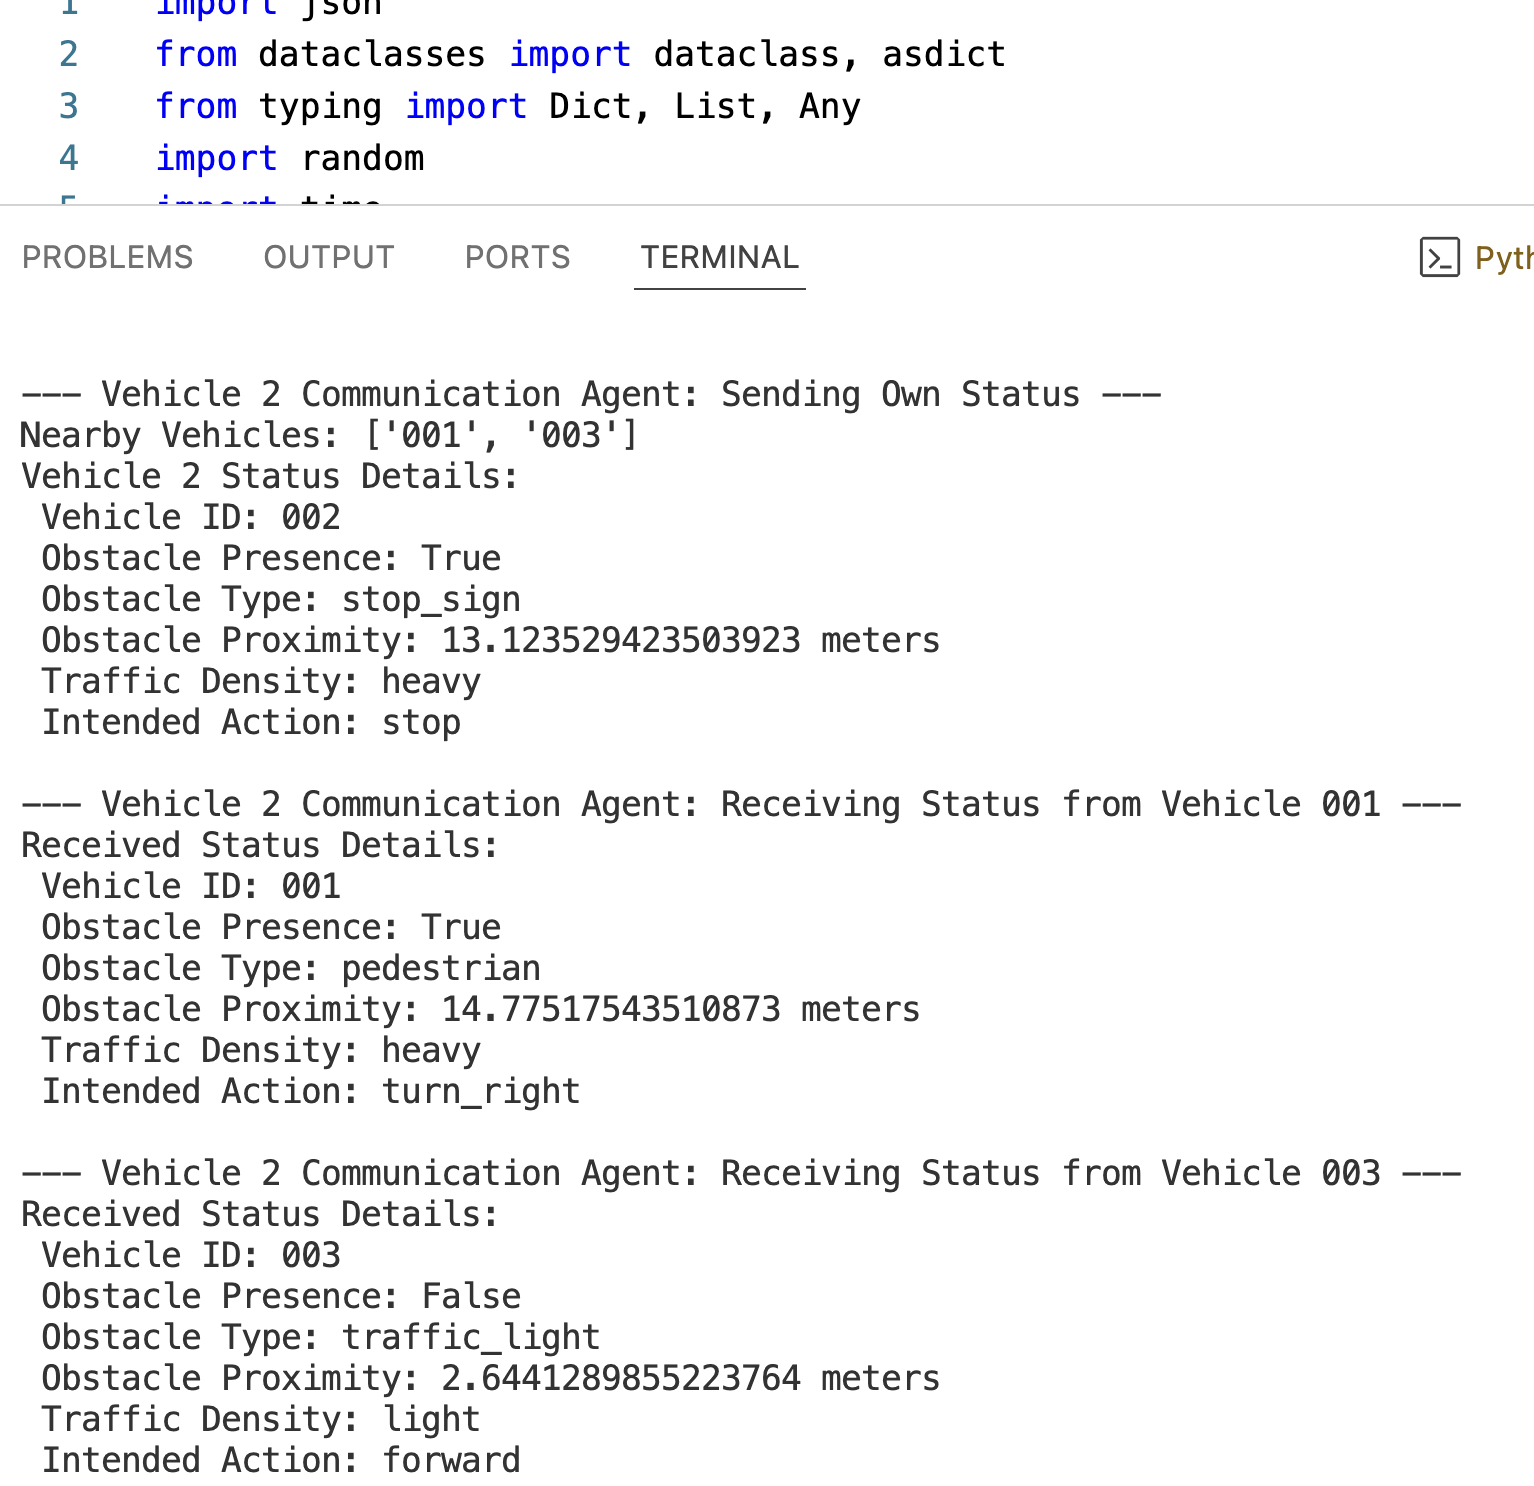
\includegraphics[width=\linewidth]{Fig/Commu_Agent.png}
     \caption{An illustration of Communication Agent}
     \label{fig:enter-label}
 \end{figure} 
For initial testing, we selected a basic traffic scenario involving an autonomous vehicle (AV) approaching a green traffic light, as illustrated in Fig. 4(a), and presented it to various language models to evaluate their decision-making behavior. The scenario was communicated through the prompt: `What would the AV on the above do? Please just answer STOP or FORWARD.' The selected models included Claude\footnote{https://claude.ai/chats} 3.7 Sonnet, GPT\footnote{https://chat.openai.com/}-4 Turbo, Falcon\footnote{https://chat.falconllm.tii.ae/} 3 7B and open-source alternatives such as OpenHermes-2.5-Mistral-7B and google/flan-t5-large. The responses of these models, sourced from Hugging Face, LM Studio, and commercial providers, are shown in Fig. 11. GPT-4 Turbo and Falcon provided direct and expected responses `FORWARD', which aligns with the logic of the situation. However, Claude deviated from the expected format by including an explanatory response, despite the prompt requesting a one-word answer. OpenHermes-2.5 responded with a clear `FORWARD', demonstrating alignment with the input instructions. Surprisingly, the google/flan-t5-large output differed from all others by responding `STOP', contradicting the intended logic of the scenario.

 \begin{figure}[b]
     \centering
     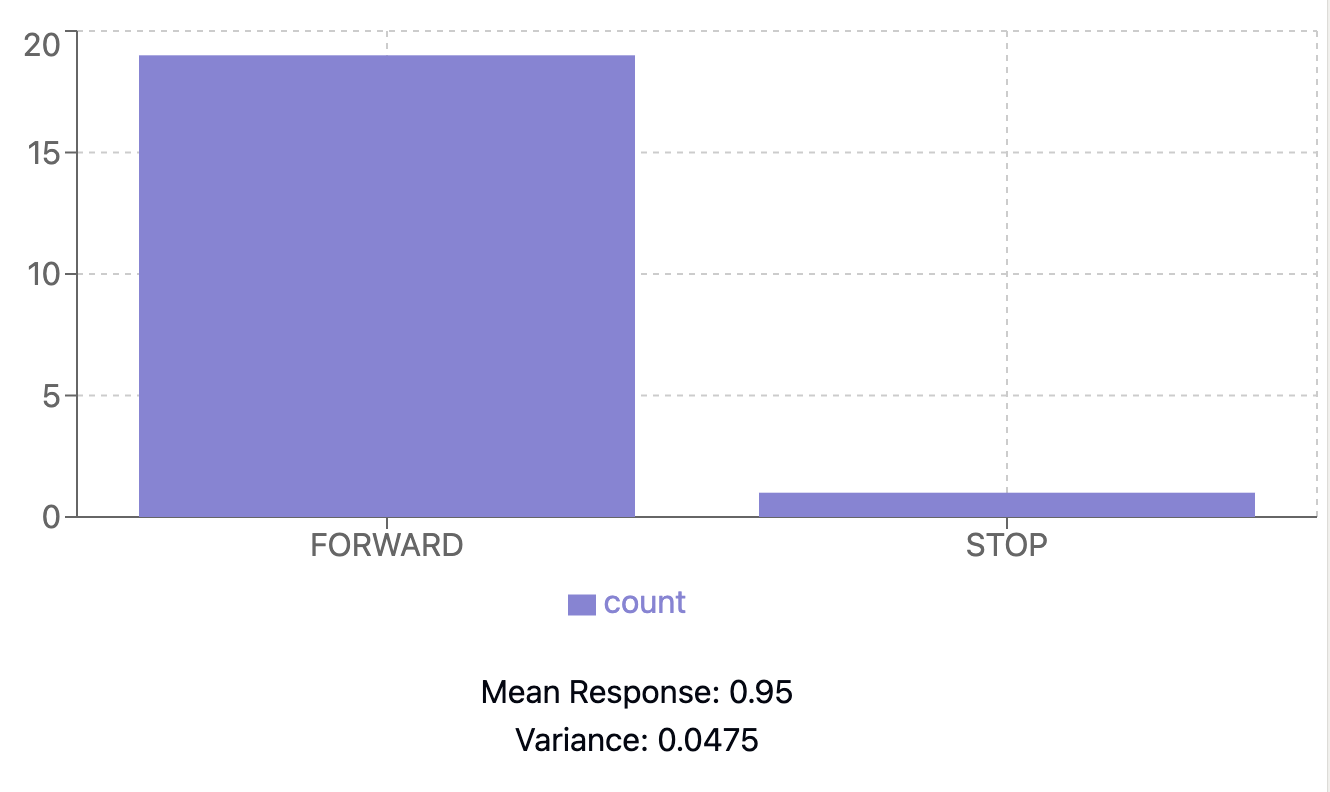
\includegraphics[width=\linewidth]{Fig/chart.png}
     \caption{LLM Model Consistency on the Tested Scenario}
     \label{fig:enter-label}
 \end{figure}
 
A major consideration was consistency. The subresearch question, `Does repeated querying of LLMs on the same scenario lead to variations in decision-making outcomes?'  will be one of such investigations of consistency.  To test this, each scenario was submitted to the models multiple times for regenerating the outputs. This approach allowed us to observe whether the models produced stable and repeatable responses or if their decisions varied unpredictably. Consistency is especially critical in autonomous vehicle (AV) applications, where uncertain output can cause serious safety concerns. 

For giving an example of this analysis, we ran the prompt at least 20 times on OpenHermes-2.5-Mistral-7B, and the consistency results are presented in Fig. 6. Consistency was calculated by mapping `FORWARD' = 1 and `STOP' = 0. `FORWARD' mean is closer to 1, it indicates that the output is having greater consistency with the expected response.

 \begin{figure}[h]
     \centering
     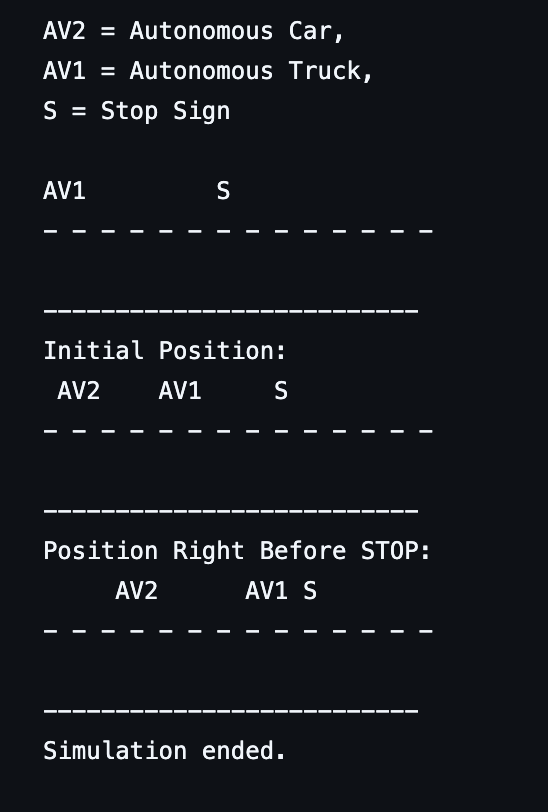
\includegraphics[width=.8\linewidth]{Fig/Communication_agent.png}
     \caption{Extended Traffic Scenario with V2V Communication }
     \label{fig:enter-label}
 \end{figure}
 % In this updated simulation scenario, AV2 (an autonomous car) is driving behind AV1 (an autonomous truck). There is a stop sign (S) ahead, but AV2 cannot see it because its line of sight is blocked by the larger AV1. For this situation, the decision from  gpt-4-turbo is `FORWARD', which could cause an accidental situation, as shown in Fig. 8.
To investigate the impact of V2V communication on autonomous decision-making, we extended our simulation to a more complex traffic scenario. In this extended scenario, AV2 (an autonomous car) follows AV1 (an autonomous truck), with a stop sign ahead that AV2 cannot see because its line of sight is blocked by AV1, as shown in Fig. 7.
 \begin{figure}[!ht]
     \centering
     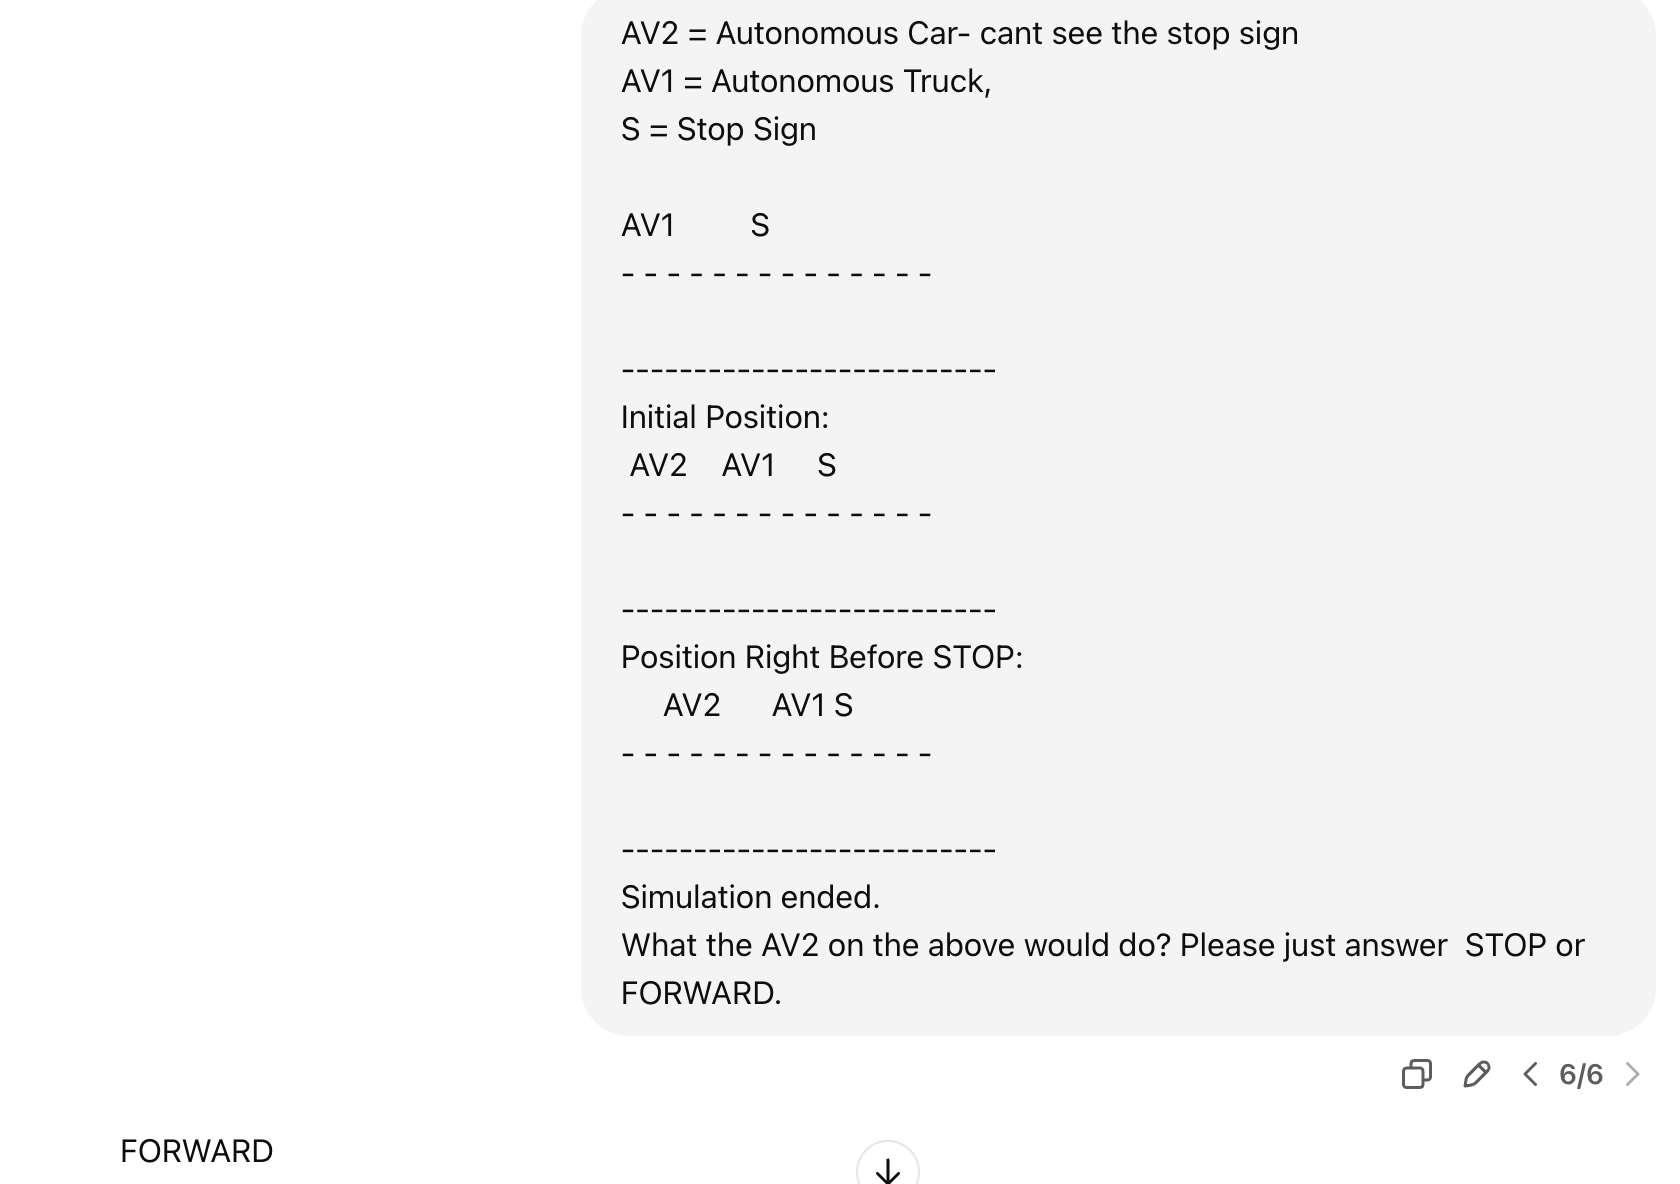
\includegraphics[width=\linewidth]{Fig/Without_communicationafent.png}
     \caption{LLM Model response without Communication agent's information (GPT-4 Turbo)}
     \label{fig:enter-label}
 \end{figure}
To investigate how LLMs process and utilize this information, this scenario was presented to the LLM with the same prompt: `What would the AV on the above do? Please, just answer STOP or FORWARD'. The model responded with `FORWARD', as shown in Fig. 8, for the case of using GPT-4 Turbo. This decision could potentially lead to an accident. 
% Without communication support, AV2 lacks the critical information needed to make a safe decision in this situation.
\begin{figure}[h]
     \centering
     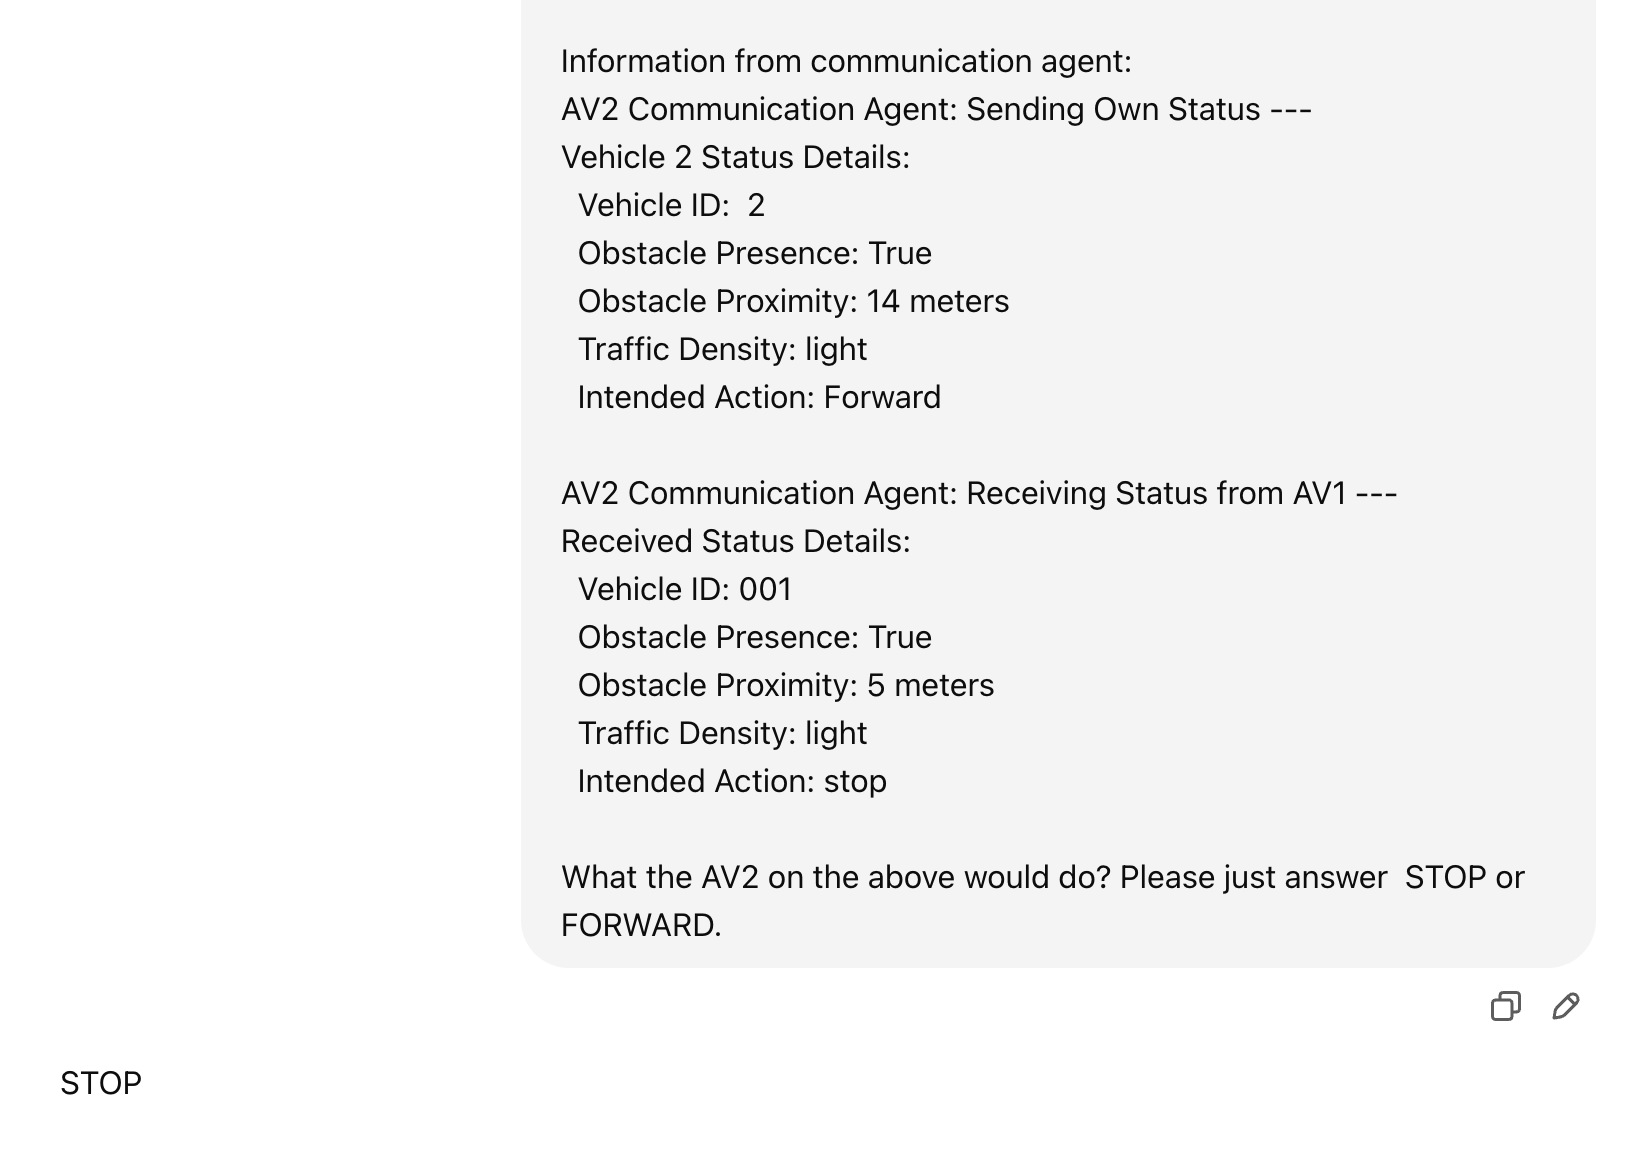
\includegraphics[width=\linewidth]{Fig/withcommunicationagent.png}
     \caption{LLM Model response with Communication agent's information (GPT4-Turbo)}
     \label{fig:enter-label}
\end{figure} 
We then examine whether the incorporation of V2V exchanged data improves the accuracy of the decisions and enables AVs to make more precise and context-aware decisions. By enabling the Communication Agent, AV1 shares its intended action and information about the obstacle ahead with AV2. These data are structured and passed as additional input presented to the model, as shown in Fig. 9, for the case of using GPT-4 Turbo. With access to this contextual information, the model responds with `STOP', even without direct visual confirmation of the traffic sign in the case where GPT-4 Turbo was used. 
\begin{figure}[!ht]
     \centering
     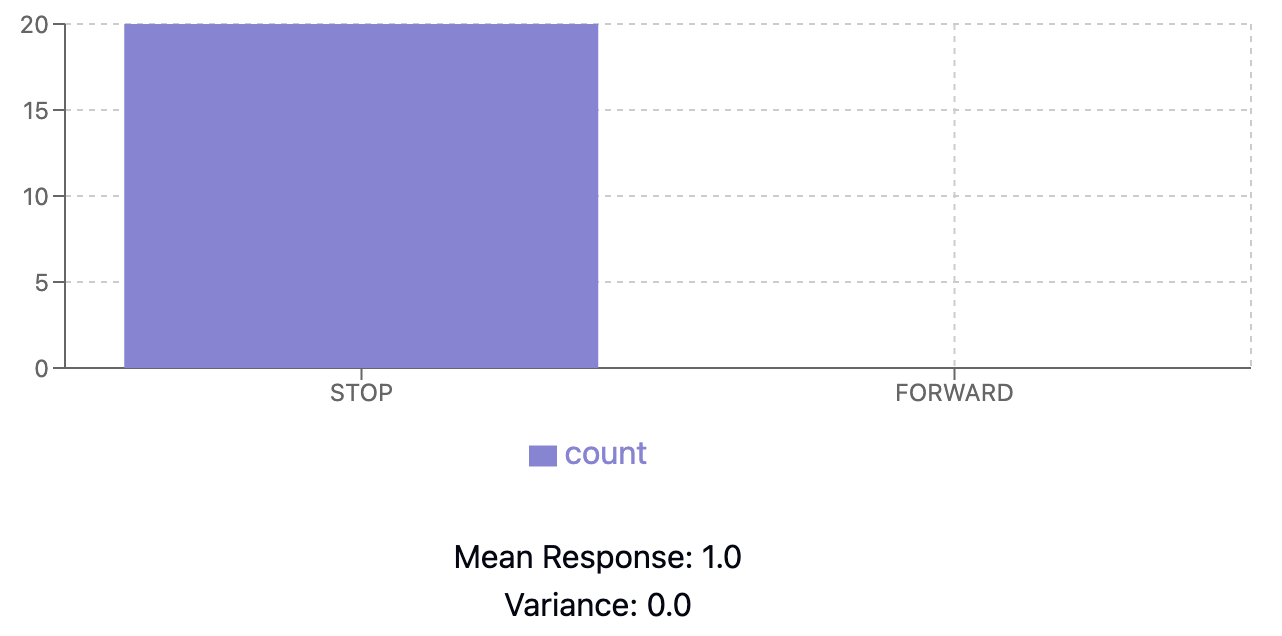
\includegraphics[width=\linewidth]{Fig/mean_wtihCA.png}
     \caption{LLM Model Consistency with V2V Communication support (GPT4-Turbo) }
     \label{fig:enter-label}
\end{figure}

To evaluate the consistency of the model decision, we ran the same prompt 20 times. The consistency was calculated by mapping `FORWARD' = 1 and `STOP' = 0. The resulting mean value of 1 for `STOP' indicates that the output is having greater consistency with the expected response. The consistency of GPT4-Turbo's responses with V2V support is shown in Fig. 10, which confirms that communication agent inputs help LLMs generate more accurate decisions in critical traffic environments.


% To address the limitations of traditional autonomous driving systems in unfamiliar or ambiguous environments, we propose a multi-agent framework that leverages the reasoning capabilities of Large Language Models (LLMs). This framework is composed of several distinct agents, with the primary focus on the Decision Agent and the Communication Agent.

% The Decision Agent is responsible for interpreting driving scenarios and selecting appropriate actions using LLMs. Instead of relying on fixed rules or pre-trained policies, it formulates text-based prompts based on environmental context and queries an LLM to infer appropriate decisions. This approach supports flexible reasoning in long-tail and previously unseen scenarios, allowing the system to respond in a human-like manner.

% A core component supporting this architecture is the Communication Agent, which facilitates standardized vehicle-to-vehicle (V2V) communication within a defined radius. When a vehicle enters the communication range of another, it exchanges structured information such as obstacle detection, speed, traffic conditions, and intended maneuvers. This data is formatted consistently, as illustrated in Fig.~6. The structured exchange allows the Decision Agent to process a richer context, enhancing decision quality and ensuring a more holistic understanding of the driving environment.

% To evaluate the consistency and reliability of the selected LLMs, we designed a set of scenario-based prompts reflecting realistic traffic situations. In one such test, the prompt described an autonomous vehicle approaching a green traffic light and asked the model to respond with either “FORWARD” or “STOP.” This test was repeated 20 times per model, and consistency was quantified by translating outputs into binary values: “FORWARD” was mapped to 1, and “STOP” to 0. The average value was then computed, as shown in Fig.~5. A mean close to 1.0 indicated consistent “FORWARD” responses, while values near 0.5 or lower suggested inconsistency or misalignment with the expected action.

% Further scenario analysis is presented in Fig.~7, which displays responses from different LLMs to a more complex scenario involving partial road blockage. The results highlight that top-tier models such as GPT-4, DeepSeek-V3, and ChatGPT exhibited consistent and accurate behavior aligned with human expectations. Conversely, some models like google/flan-t5-large demonstrated less predictable responses, occasionally deviating from the intended logic or including verbose explanations despite the prompt requesting a concise answer.

% These observations support a key insight of our approach: desirable performance from LLMs can be expected when certain operational conditions are met. Specifically, models perform best when prompted with well-structured, context-rich inputs and confined to bounded decision-making tasks. To operationalize this, our framework includes a pre-processing layer that transforms V2V communication data into structured textual inputs optimized for LLM reasoning.

% Together, these elements define a scalable, interpretable, and adaptive framework for autonomous decision-making, capable of integrating structured sensory data with high-level reasoning to navigate complex driving scenarios.


\section{Conclusion}
We presented an approach for leveraging Large Language Models (LLMs) to enhance reasoning capabilities in uncertain traffic situations within a multi-agent framework for autonomous vehicles. We have investigated LLMs from Hugging Face, LM Studio, as well as major commercial services such as Claude, GPT-4 Turbo, and Falcon. Their responses to basic traffic scenarios were analyzed, revealing varying levels of consistency and accuracy. These results reveal both the promise and the current limitations of this approach, highlighting the need for improved consistency in the model responses. The proposed approach aims at the realization of adaptive autonomous systems capable of human-like reasoning in unpredictable situations. By integrating contextual data derived from V2V communication with LLM reasoning, our goal is to bridge the critical gap in decision-making accuracy for autonomous vehicles.


% final page output

\begin{figure*}[h]
    \centering
    % First Row
    \begin{subfigure}[b]{0.48\textwidth}
        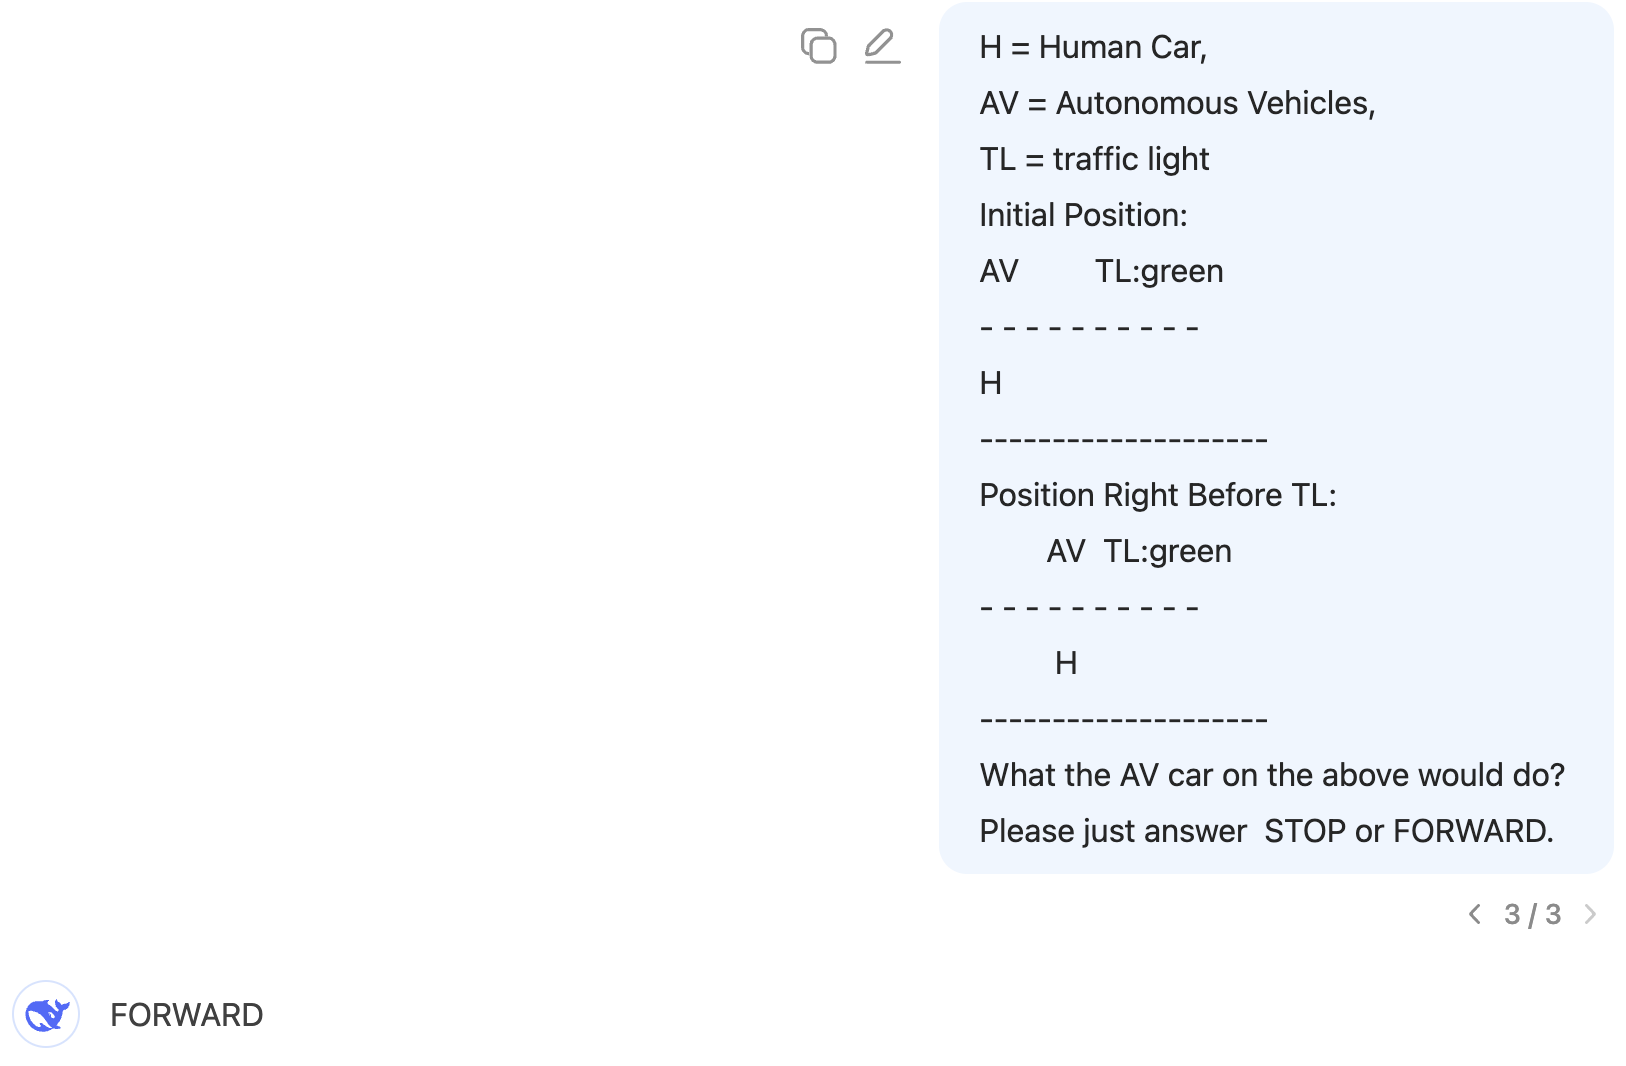
\includegraphics[width=\linewidth]{outfromLLM/DeepSeek.png}
        \caption{Output from DeepSeek-V3}
    \end{subfigure}
    \hfill
    \begin{subfigure}[b]{0.48\textwidth}
        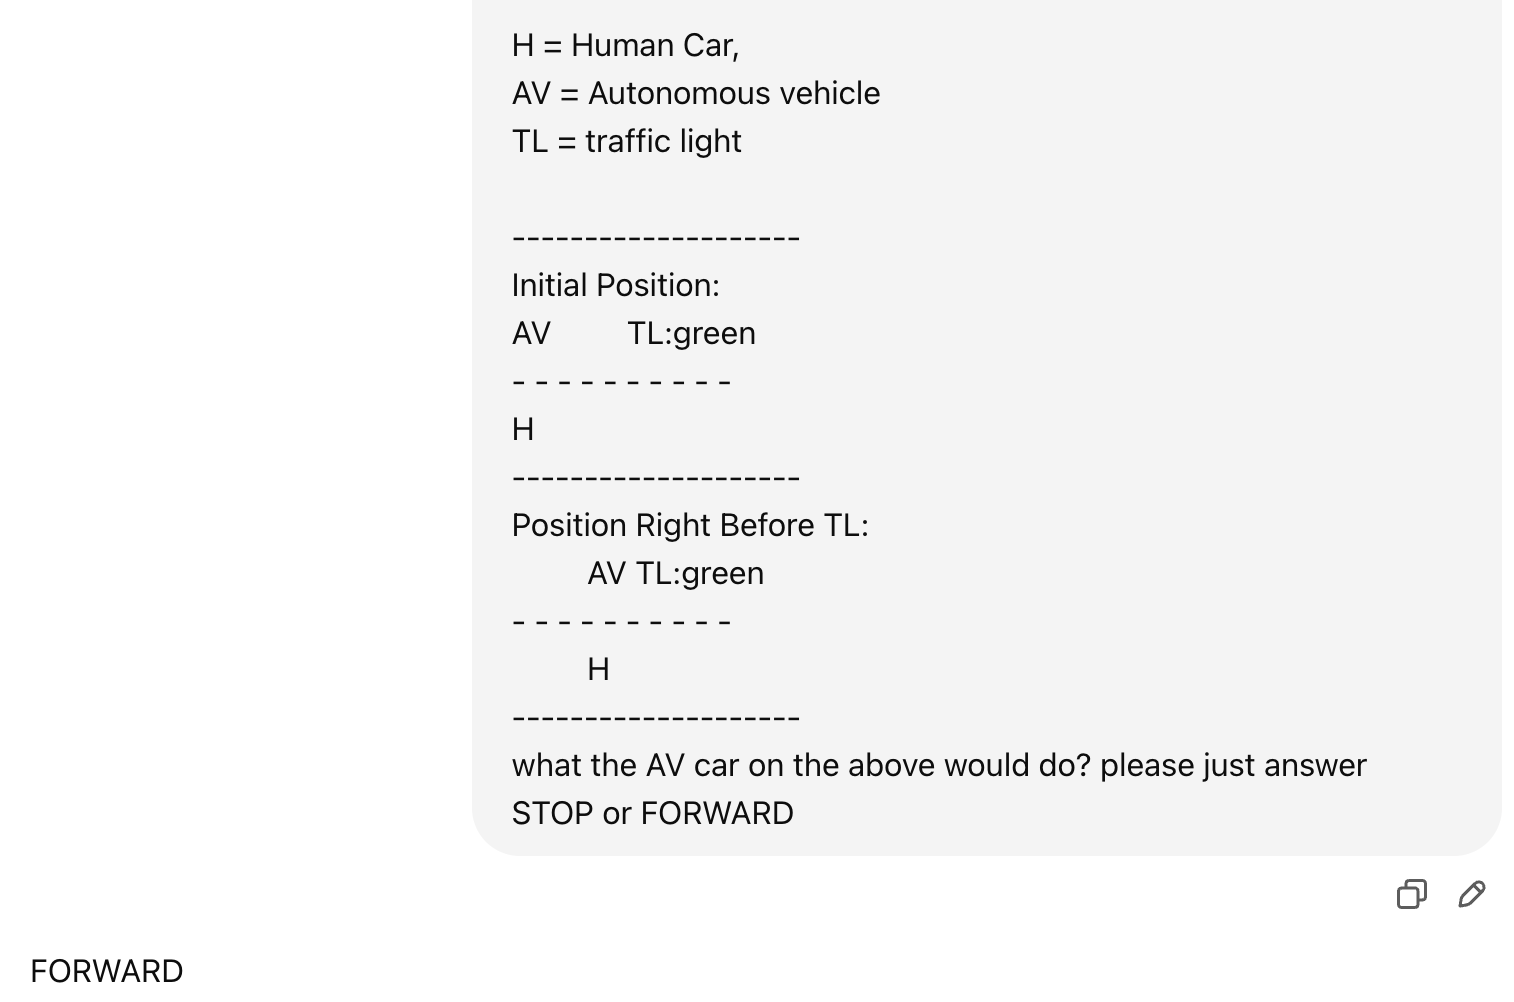
\includegraphics[width=\linewidth]{outfromLLM/GPT.png}
        \caption{Output from gpt-4-turbo}
    \end{subfigure}
    
    \vspace{1em}
    \begin{subfigure}[b]{0.48\textwidth}
        \includegraphics[width=\linewidth]{outfromLLM/claude.png}
        \caption{Output from Claude 3.7 Sonnet}
    \end{subfigure}
    % Space between rows
    \hfill
    % Second Row
    \begin{subfigure}[b]{0.48\textwidth}
        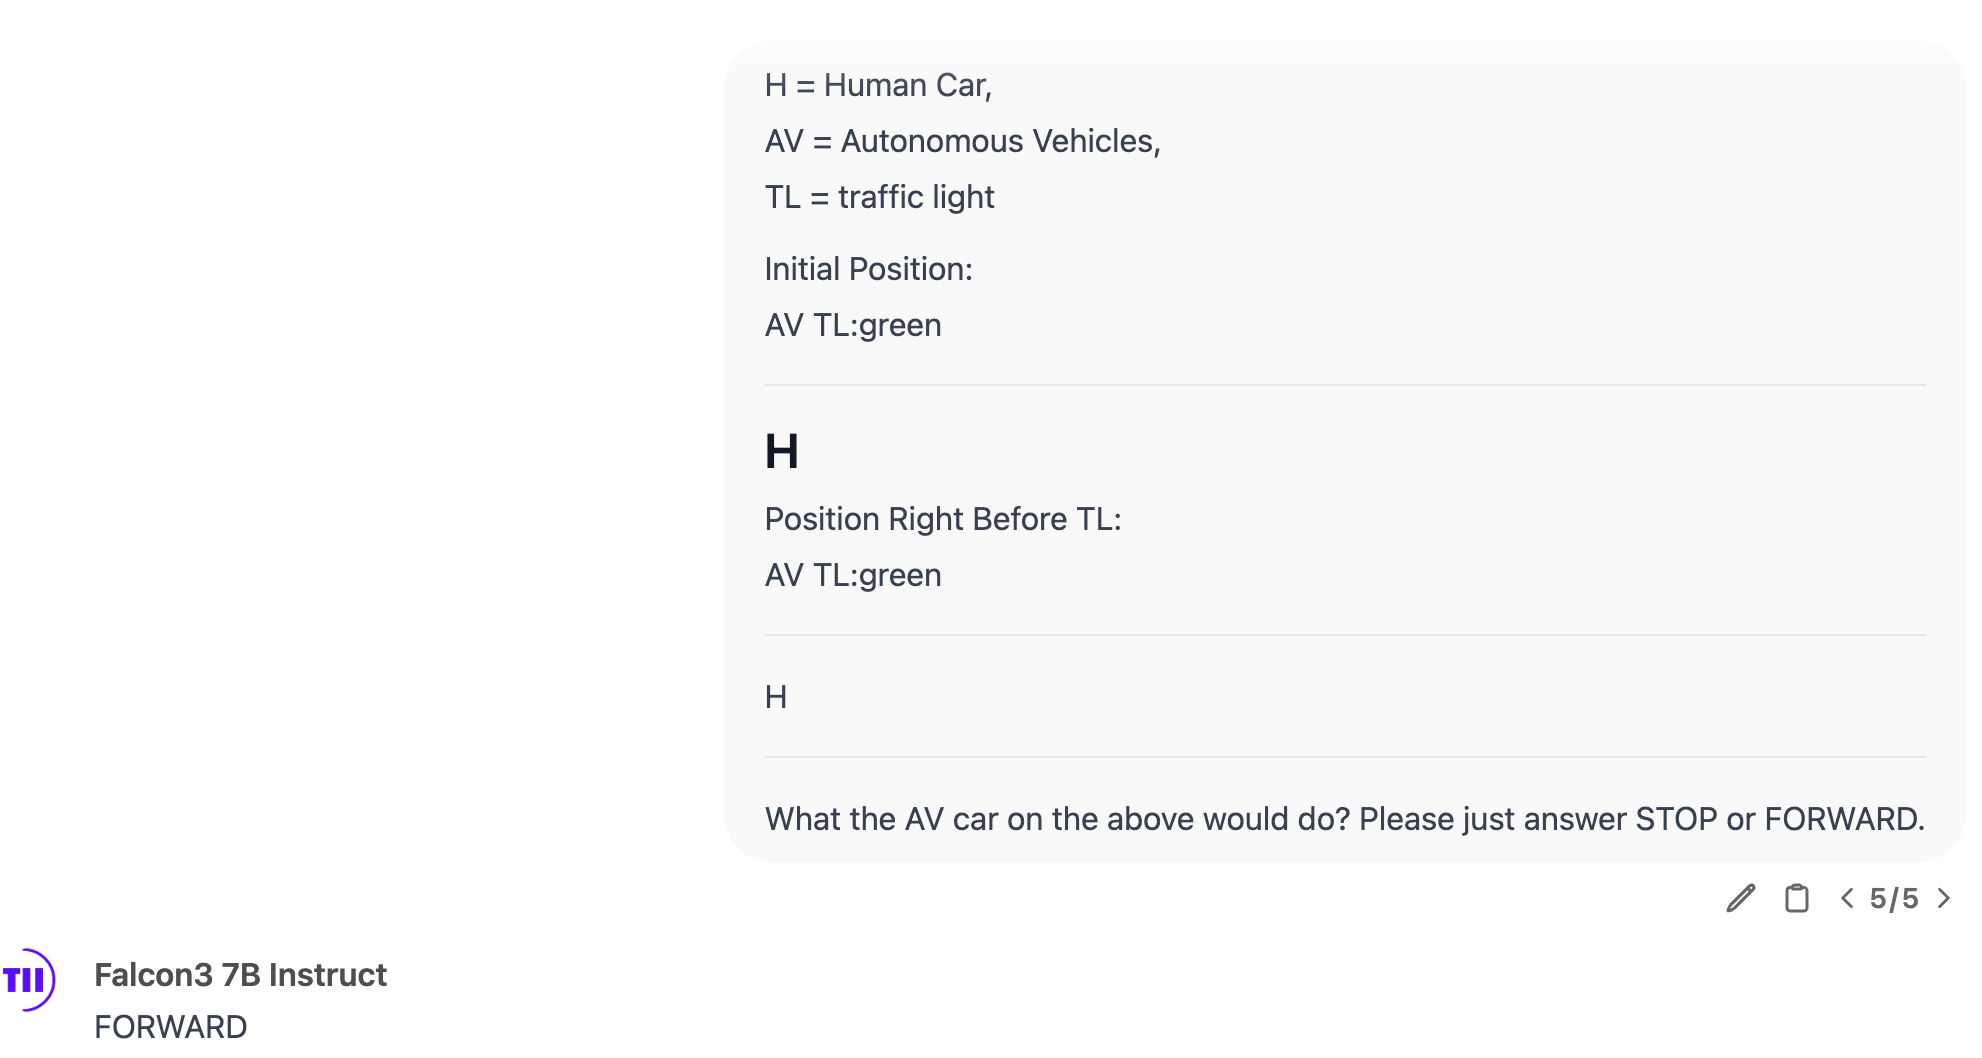
\includegraphics[width=\linewidth]{outfromLLM/Falcon3.png}
        \caption{Output from Falcon3 7B}
    \end{subfigure}
    \vspace{1em}
    \begin{subfigure}[b]{0.48\textwidth}
        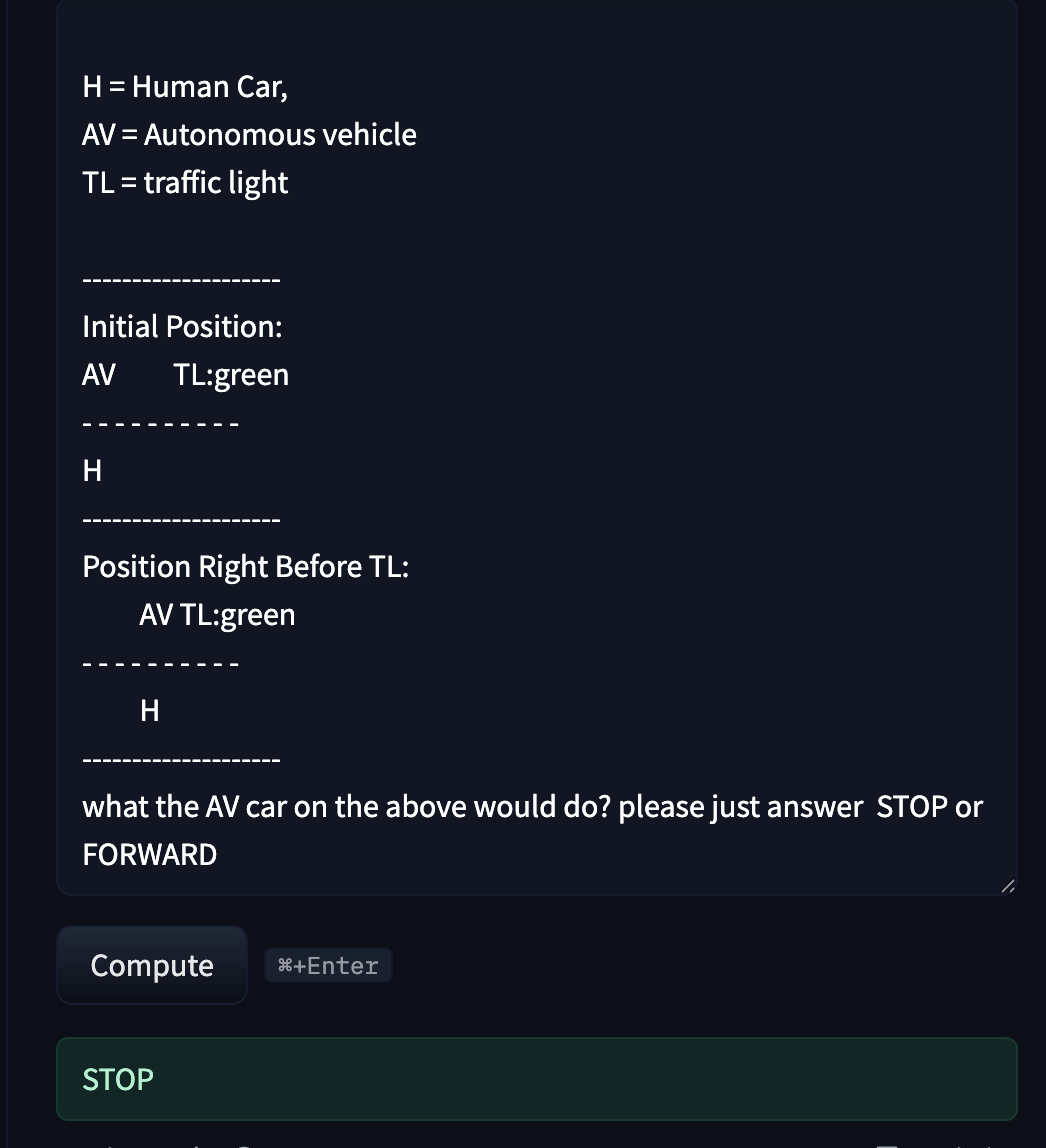
\includegraphics[width=\linewidth]{outfromLLM/google:flan-t5-large.png}
        \caption{Output from google/flan-t5-large}
    \end{subfigure}
    \hfill
    \begin{subfigure}[b]{0.48\textwidth}
        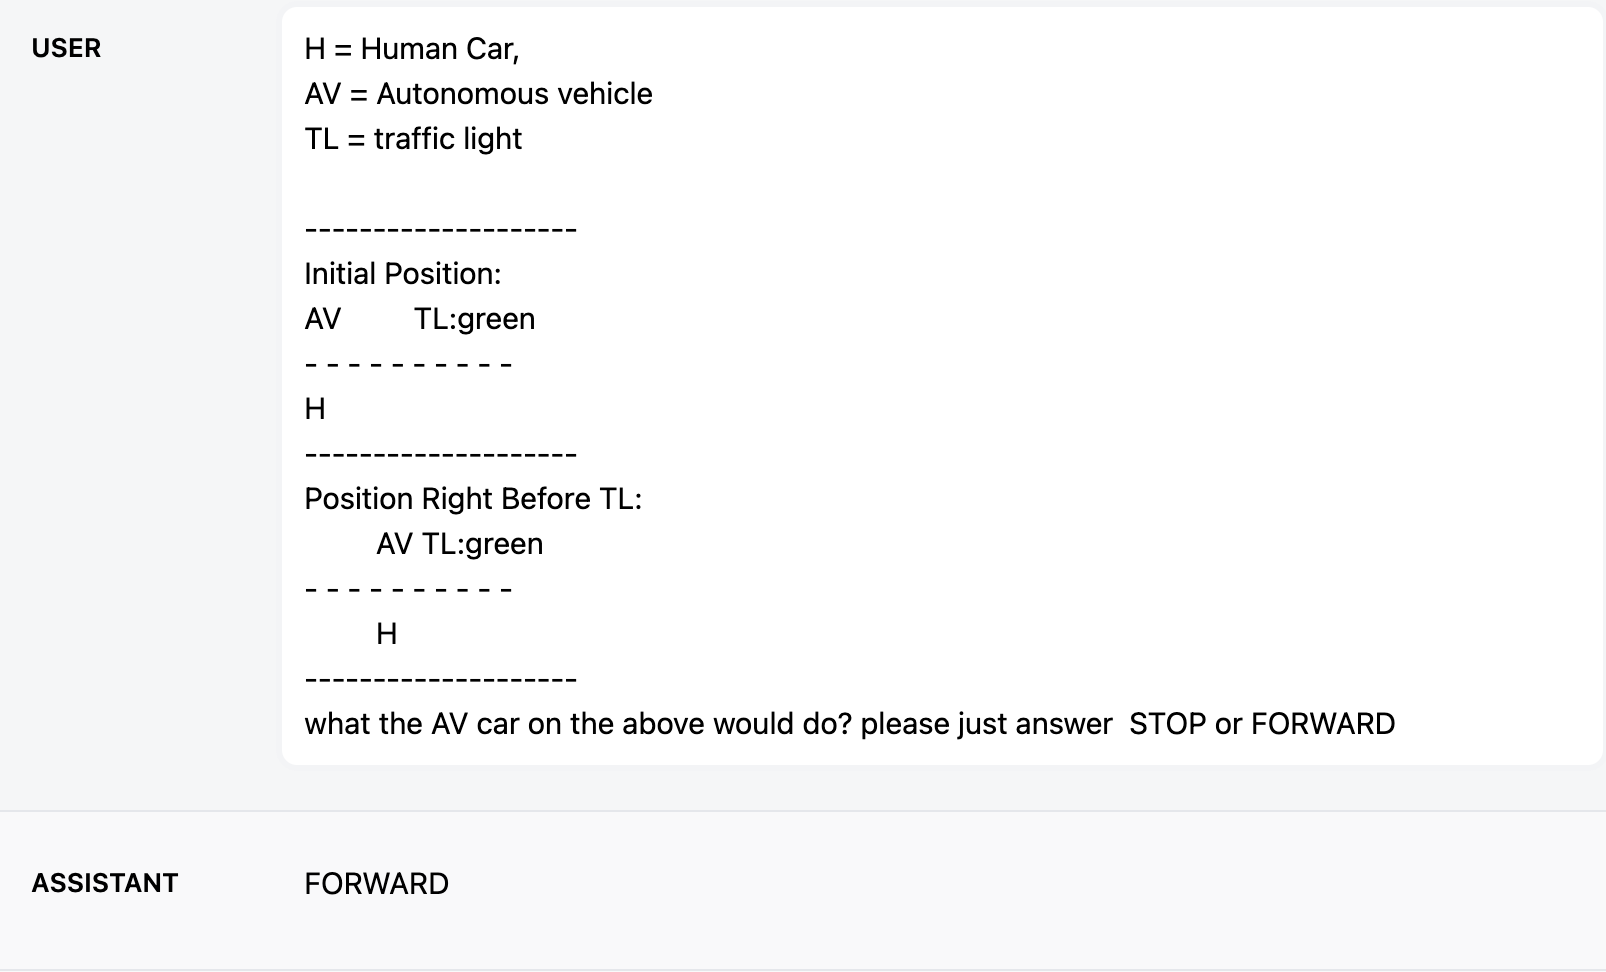
\includegraphics[width=\linewidth]{outfromLLM/FROM_LLM.png}
        \caption{Output from OpenHermes-2.5-Mistral-7B}
    \end{subfigure}

    \caption{Responses from different LLMs}
    \label{fig:llm_outputs}
\end{figure*}




% \clearpage
% this is the reference part
\bibliographystyle{ieeetr}
\bibliography{references}
\end{document}


